\documentclass[12pt]{article}
\usepackage{amsmath}
\usepackage{graphicx}
\usepackage{amsfonts}
\usepackage{hyperref}
\usepackage{geometry}
\usepackage{listings} 
\usepackage{placeins}
\usepackage[T1]{fontenc}

\geometry{top=2.5cm, bottom=2.5cm, left=2.5cm, right=2.5cm}

\title{Signal Synthesis Using Inverse Discrete Fourier Transform (IDFT)}
\author{Daria Kręcichwost}
\date{\today}

\begin{document}

\begin{titlepage}
    \centering
    \vspace*{2cm}
    
    \Huge
    REPORT
    
    \vspace{1cm}
    
    \Large
    Course: Analog and digital electronic circuits \\
    Teacher: Prof. Dr. Hab. Vasyl Martsenyuk
    
    \vfill
    
    \Large
    Lab No. \\
    Date: \today \\
    Topic: "" \\
    Variant: 8
    
    \vspace{1cm}
    
    \large
    Name: Daria Kręcichwost \\
    Computer Science (Second Degree) \\
    Part-time studies, Semester 1 \\
    Group: B
\end{titlepage}

\newpage

\maketitle


\section{Problem Statement}


\section{Input Data}


\section{Commands used (or GUI)}


\begin{lstlisting}[language=Python, breaklines=true]
code

\end{lstlisting}
\item \href{https://github.com/DariaKrecichwostQA/StudiaUBB/tree/main/Digital%20Signal%20Processing/Zad1}{{Link to remote repository on GitHub})}

\newpage
\section{Outcomes}


\subsection{Real Part of the Signal}

\vfill
\newpage
\subsection{text)}
\begin{figure}[htbp]
    \centering
    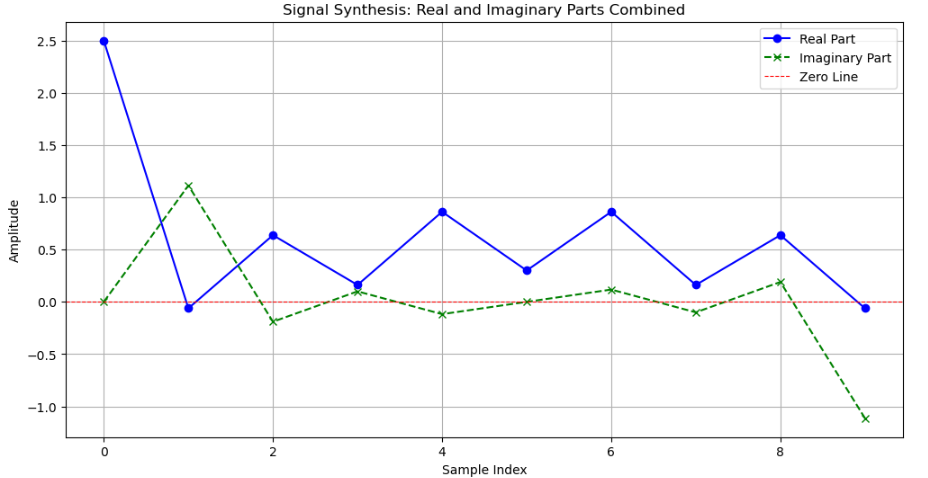
\includegraphics[width=0.8\textwidth]{3.png}
    \caption{Text}
    \label{fig:text}
\end{figure}

\FloatBarrier
\vfill


\newpage

\section{Conclusions}

\begin{itemize}
    \item 
\end{itemize}



\end{document}
